\documentclass[twocolumn,times]{aastex631}
\usepackage{acronym}

% \received{March 1, 2021}
% \revised{April 1, 2021}
% \accepted{\today}
% \submitjournal{AJ}
\shorttitle{M$^4$OPT}
\shortauthors{Singer et al.}

% Some of these acronym definitions contain the definite article ("the") and some do not.
% If an acronym's part of speech is a proper noun, then it has a definite article when it
% appears in expanded form. For example, we write "The UltraViolet Explorer is a space telescope,"
% and "UVEX is a space telescope," but we don't write "The luminosity function of the kilonovae is given in Eq. (3)."
\acrodef{ACCESS}[ACCESS]{Advanced Cyberinfrastructure Coordination Ecosystem: Services \& Support}
\acrodef{CDF}[CDF]{cumulative distribution function}
\acrodef{CSR}[CSR]{concept study report}
\acrodef{FOV}[FOV]{field of view}
\acrodef{GRB}[GRB]{gamma-ray burst}
\acrodef{GW}[GW]{gravitational wave}
\acrodef{KN}[KN]{kilonova}
\acrodefplural{KN}[KNe]{kilonovae}
\acrodef{LIGO}[LIGO]{the Laser Interferometer Gravitational-Wave Observatory}
\acrodef{MIDEX}[MIDEX]{Medium-Class Explorer}
\acrodef{M4OPT}[M$^4$OPT]{the Multi-Mission Multi-Messenger Observation Planning Toolkit}
\acrodef{NOSA}[NOSA]{the NASA Open Source Agreement}
\acrodef{NS}[NS]{neutron star}
\acrodef{NSF}[NSF]{the U.S. National Science Foundation}
\acrodef{NUV}[NUV]{near ultraviolet}
\acrodef{FUV}[FUV]{far ultraviolet}
\acrodef{PSF}[PSF]{point spread function}
\acrodef{ROI}[ROI]{region of interest}
\acrodef{SN}[SN]{supernova}
\acrodefplural{SN}[SNe]{supernovae}
\acrodef{S/N}[S/N]{signal to noise ratio}
\acrodef{SDSC}[SDSC]{the San Diego Supercomputing Center}
\acrodef{ToO}[ToO]{target of opportunity}
\acrodefplural{ToO}[ToOs]{targets of opportunity}
\acrodef{UV}[UV]{ultraviolet}
\acrodef{UVEX}[UVEX]{the UltraViolet EXplorer}

\begin{document}

\title{Mixed Integer Linear Programming for Time-Domain and Multimessenger Observation Scheduling}

\author[0000-0001-9898-5597]{Leo P. Singer}
\affiliation{Astroparticle Physics Laboratory, NASA Goddard Space Flight Center}
\email{leo.p.singer@nasa.gov}

\author{Friends}

\begin{abstract}
\Ac{UVEX} is a wide-field, all-sky, time-domain, ultraviolet survey space telescope selected as a NASA \ac{MIDEX} mission for launch in 2030. \ac{UVEX} will conduct an unprecedented all-sky time-domain survey in two \ac{UV} filters. \ac{UVEX} will follow up \ac{GW} binary neutron star mergers as \acp{ToO}, rapidly scanning across their localization regions to search for their \ac{KN} counterparts. Early-time multiband ultraviolet light curves of \acp{KN} are key to explaining the interplay between jet and ejecta in binary neutron star mergers. Owing to high Galactic extinction in the ultraviolet and \ac{UVEX}'s large \ac{FOV}, variation in sensitivity across the \ac{GW} \ac{ROI} is an important consideration for observation planning. We present an adaptive strategy for \ac{GW} follow-up with \ac{UVEX} in which exposure time is adjusted dynamically for each field individual to maximize the overall probability of detection. We have implemented this strategy in an open source astronomical scheduling toolkit called \ac{M4OPT}, on GitHub at \url{https://github.com/m4opt/m4opt}.
\end{abstract}

\keywords{Computational methods~(1965) --- Gravitational wave astronomy~(675) --- Open source software~(1866) --- Ultraviolet observatories~(1739) --- Ultraviolet transient sources~(1854) --- Wide-field telescopes~(1800)}

\acresetall

\section{Introduction} \label{sec:intro}

In 2017, \ac{LIGO} and Virgo \citep{2017PhRvL.119p1101A} detected a long-duration \ac{GW} inspiral signal, GW170817, at the same time that Fermi \citep{2017ApJ...848L..14G} and INTEGRAL \citep{2017ApJ...848L..15S} recorded a short \ac{GRB}, GRB170817a. The alert sprang traps that had been set by hundreds of telescopes worldwide \citep{2014ApJS..211....7A,2016ApJ...826L..13A} which quickly found the optical counterpart \citep{2017Sci...358.1556C}, AT2017gfo. As a measure of the degree to which the event focused the efforts of astronomers everywhere, the author list of \citet{2017ApJ...848L..12A} runs to 24 pages!

The scientific harvest from this one event was remarkable. It fulfilled a three-decaded-old dream of using \acp{GW} as ``standard sirens'' to measure the Hubble constant \citep{1986Natur.323..310S,2017Natur.551...85A}. Moreover, it proved once and for all the hypotheses that \ac{NS} mergers are the central engines of short \acp{GRB} \citep{2013ApJ...776...18F} and the main cosmic factories of heavy $r$-process elements \citep{1999ApJ...525L.121F}. 

It had long been understood that such mergers would tidally disrupt their \acp{NS}, and that radioactive decay of the heavy elements synthesized in their hot neutron-rich ejecta would fuel transients \citep{1974ApJ...192L.145L,1989Natur.340..126E,1998ApJ...507L..59L} that came to be called \acp{KN}. In those early days, people assumed that the ejecta would have opacities similar to those in \acp{SN} and predicted fairly bright \ac{KN} light curves that peaked in the optical or \ac{UV} and that would be fairly easy to detect. However, further study of the atomic structure of lanthanides led to the realization that their dense absorption spectra would lead to line-blanketing in the optical, containing the radiation and only letting it leak out much more slowly and at longer wavelengths, in the infrared \citep{2013ApJ...774...25K}. Observers grimly realized that although \acp{KN} were still among the most promising counterparts of \ac{NS} mergers \citep{2012ApJ...746...48M}, they would be much dimmer, redder, and harder to detect than previously expected.

Although these later and more sober predictions agreed remarkably well with the observed spectral sequence of AT2017gfo \citep{2017Natur.551...67P,2017Natur.551...80K}, contrary to those expectations it was quite blue and featureless at the earliest observed times \citep{2017Sci...358.1574S}. In the fallout from GW170817, the cause of this early optical and \ac{UV} emission remains one of the most enduring mysteries. The blue emission could be radioactively powered but result from a geometrically distinct outflow component with higher velocity and/or lower lanthanide fraction \citep{2017ApJ...848L..18N} or could result from the shock caused by the ``cocoon'' interaction between the ejecta and the nascent jet \citep{2017Sci...358.1559K,2018MNRAS.479..588G}. Lacking for GW170817, early-time \ac{UV} observations, less than 12 hours after merger, could handily settle the debate \citep{2018ApJ...855L..23A}.

The 2020 decal survey by the \citet{2021pdaa.book.....N} recommended that ``NASA should establish a time-domain program to realize and sustain the necessary suite of space-based electromagnetic capabilities required to study transient and time-variable phenomena, and to follow up multi-messenger events.'' Responding to this need, \ac{UVEX} \citep{2021arXiv211115608K} was recently selected as NASA's next \ac{MIDEX}, expected to launch in 2030. Both \ac{UVEX} and the Israeli-led ULTRASAT mission \citep{2024ApJ...964...74S} will fill an acknowledged gap in time-domain capability and transient discovery potential in the \ac{UV} \citep{2014AJ....147...79S}. Although \ac{UVEX} is expected to launch a few years after ULTRASAT, it has several advantages: it will take images simultaneously in two bands, it will observe much deeper ($>$25.8~mag over the entire survey), it will have a \ac{PSF} that is well-matched to ground-based follow-up ($\sim1\arcsec$), and it will have an onboard spectrograph.

\Ac{M4OPT} is a rewrite of dorado-scheduling\footnote{\url{https://github.com/nasa/dorado-scheduling}} and dorado-sensitivity\footnote{\url{https://github.com/nasa/dorado-sensitivity}}.

\Ac{NOSA} has been panned by the \citet{FSF}, the \citet{NAP25217}, and even the \citet{SMD}.

\begin{figure}
    \plotone{figures/uvex-tiling}
    \caption{\label{eq:fig:uvex-tiling}An example of a \ac{ToO} observation sequence with \ac{UVEX} to follow up a \ac{GW} event. Adapted from Fig.~D-8 from the \ac{UVEX} \ac{CSR} submitted to NASA Headquarters, which is also Fig.~14 in \citet{2021arXiv211115608K}.}
\end{figure}

\section{Fundamentals of mixed integer programming}

\subsection{Logic to MILP translation dictionary}

\subsection{A simple example}

\subsection{Maximum weighted coverage problem}

\subsection{No overlap constraints}

\section{Progressive elaboration of the problem}

\subsection{Tiling and scheduling without slew constraints}

\section{Case study: GW observations with UVEX}

Here is the setup of our case study.

\paragraph{\Ac{GW} localizations}
We started with the same simulated \ac{GW} localizations as \citet{criswell}, which covers LIGO, Virgo, and KAGRA's fifth~(O5) and sixth~(O6) observing runs. The data are publicly archived in \cite{r_weizmann_2024_14142970}. These simulated events were generated using the same methodology as \citet{2022ApJ...924...54P} and \citet{2023ApJ...958..158K}, except that the \ac{S/N} threshold for \ac{GW} detection is set to~10. The localizations were generated with the rapid localization engine BAYESTAR \citep{2016PhRvD..93b4013S} and consist of 3D posterior probability distributions of sky location and luminosity distance \citep{2016ApJ...829L..15S,2016ApJS..226...10S}.

\paragraph{\Ac{KN} absolute magnitude}
Appendix~E.2 of \citet{2021arXiv211115608K} specifies fiducial parameter ranges for radioactively-powered or shock-powered \ac{KN} models and 90\% credible intervals for the absolute magnitude in each band. These absolute magnitude ranges are reproduced in the Table~\ref{tab:kn-abs-mag} below. \ac{UVEX} obseves in both the \ac{NUV} and \ac{FUV} filters simultaneously. In orer to achieve a detection in at least one filter, regardless of the model, we should plan obsevations using the fainter of the two models and the brighter of the two bands: the nucleosynthesis-powered model in NUV, with an absolute magnitude range of $[-15.6, -12.4]$. Assuming that this is the 90\% credible interval of a Gaussian distribution, the absolute magnitude has the approximate distribution
%
\begin{equation}
    M_\mathrm{NUV} \sim \mathcal{N}(-14, 1).
\end{equation}

\begin{deluxetable}{lcc}
    \tablecaption{\label{tab:kn-abs-mag}Ranges of peak absolute magnitudes of \acp{KN}. Adapted from \citet{2021arXiv211115608K} Appendix E.2.}
    \tablehead{
        & \multicolumn2c{absolute magnitude range} \\
        \colhead{Model} & \colhead{NUV} & \colhead{FUV}
    }
    \startdata
    Nucleosynthesis powered & [-15.6, -12.4] & [-17.8, -15.3] \\
    Shock powered & [-14.5, -10.2] & [-17.9, -15.0]
    \enddata
\end{deluxetable}

\paragraph{Follow-up time window}
\citet{criswell} required a single epoch of \ac{UVEX} observations to take 3~hours or less. To match this choice, we configure \ac{M4OPT} to plan two visits of each field with a minimum cadence of 30~min between repeated visits, with a total elapsed time limit of 6~hours. 

\paragraph{Exposure time}
The exposure time is allowed to vary adaptively for each field, with a minimum exposure time of $\epsilon_\mathrm{min} = 300$~s. The minimum exposure time corresponds to a single standard \ac{UVEX} imaging exposure. (A standard survey dwell consists of 3 consecutive stacked 300~s exposures.)

\paragraph{Run duration}
As in \citet{criswell}, we assumed 1.5~years of overlap between the \ac{UVEX} prime mission and the \ac{GW} observing run.

\paragraph{Follow-up selection criterion}
We ran \ac{M4OPT} on all simulated events. We considered events selected for follow-up with \ac{UVEX} if the scheduler's objective values $P$ was less than $P^* = 0.1$. Although the decision of whether to execute a \ac{ToO} is based solely on the scheduler's objective value, we can predict an analytical threshold for triggering on an event based on the area of its $Q$th credible region and its luminosity distance $d_\mathrm{L}$:
%
\begin{eqnarray}
    d_\mathrm{L} &<& d_\mathrm{L}^* = 10^{\frac{1}{5}(x^* - \mu_X + \sigma_X \Phi^{-1}(1-P^*) - 25)}\,\mathrm{Mpc} \label{eq:threshold-distance} \\
    A_Q &<& A_Q^* = \left(\frac{\Psi^{-1}(Q)}{\Psi^{-1}(P^*)}\right)^2 \left(\frac{\delta - \beta}{\epsilon_\mathrm{min} n_K}\right)A_\mathrm{FOV} \label{eq:threshold-area} \\
    \frac{A_Q}{A_\mathrm{FOV}} &<& \left(\frac{d_\mathrm{L}}{d_\mathrm{L}^*}\right)^{-4} \label{eq:threshold-area-distance}
\end{eqnarray}
%
where $x^*$ is the faintest limiting magnitude at any point on the sky, $A_\mathrm{FOV}$ is the area of the \ac{FOV}, $\Phi(x)$ is the inverse of the \ac{CDF} of the standard normal distribution, and $\Psi^{-1}(x) = -2\ln(1 - x)$ is the inverse of the \ac{CDF} of a $\chi^2$ distribution with 2 degrees of freedom.

The results are shown in Fig~\ref{fig:area-distance}. The expected numbers of events selected for follow-up and detected are shown in Table~\ref{tab:selected-detected} below.

\begin{figure*}
    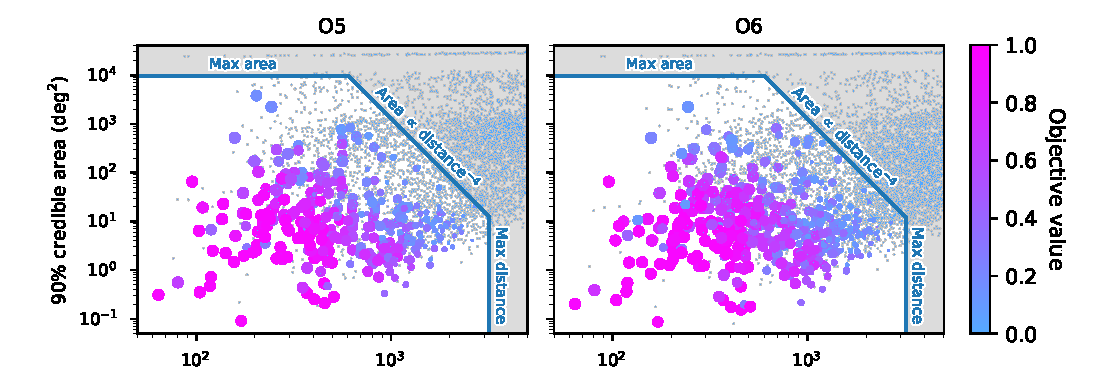
\includegraphics[width=\textwidth]{figures/area-distance}
    \caption{\label{fig:area-distance}90\% credible area and distance of simulated \ac{GW} events. Events that were selected for follow-up with \ac{UVEX} are represented by colored dots, with the color of the dot representing the scheduler objective value and the area of the dot the detection probability. Events that were not selected for follow-up are marked with gray dots. The blue boundary represents the analytical predictor of the detection threshold given by Eqs.~(\ref{eq:threshold-distance},\ref{eq:threshold-area},\ref{eq:threshold-area-distance}).}
\end{figure*}

\begin{deluxetable}{lcc}
    \tablecaption{\label{tab:selected-detected}Expected number of events selected for follow-up and detected.}
    \tablehead{& O5 & O6}
    \startdata
    Number of events selected & $51_{-31}^{+67}$ & $72_{-42}^{+93}$ \\
Number of events detected & $26_{-16}^{+35}$ & $38_{-23}^{+51}$

    \enddata
\end{deluxetable}

\section{Conclusion}

\begin{acknowledgments}
This work was performed in part at the Aspen Center for Physics, which is supported by \ac{NSF} grant PHY-2210452.

This work used Expanse at \ac{SDSC} through allocation AST200029, ``Towards a complete catalog of variable sources to support efficient searches for compact binary mergers and their products,'' from the \ac{ACCESS} program, which is supported by \ac{NSF} grants \#2138259, \#2138286, \#2138307, \#2137603, and \#2138296.
\end{acknowledgments}

\vspace{5mm}
\software{
    astropy \citep{2013A&A...558A..33A,2018AJ....156..123A},
    dust\_extinction \citep{2024JOSS....9.7023G},
    dustmaps \citep{2018JOSS....3..695M},
    HEALPix \citep{2005ApJ...622..759G},
    healpy \citep{2019JOSS....4.1298Z},
    ligo.skymap \citep{2016PhRvD..93b4013S,2016ApJ...829L..15S,2016ApJS..226...10S},
    synphot \citep{2018ascl.soft11001S}}

\bibliography{m4opt}{}
\bibliographystyle{aasjournal}

\end{document}
